\section{Statistical Properties of Control Charts}
\noindent\rule[\linienAbstand]{\linewidth}{\linienDickeDick}
Aim of process control using control charts: Keep the process under statistical control.
Or, if it is not at the beginning, to put it into statistical control by improving production conditions.



\subsection{Interpretation of Control Charts}
\noindent\rule[\linienAbstand]{\linewidth}{\linienDicke}

\subsection{Western Electric Rules}
\noindent\rule[\linienAbstand]{\linewidth}{\linienDicke}
\begin{enumerate}
  \item Any single data point falls outside the limit defined by UCL and LCL (beyond the 3$\sigma$-limit).
  \item 2. Two out of three consecutive points fall beyond the limit defined by $\frac{2}{3}$ UCL and $\frac{2}{3}$ LCL on the same side of the centreline (beyond the 2$\sigma$-limit).
  \item Four out of five consecutive points fall beyond the limit defined by $\frac{1}{3}$UCL and $\frac{1}{3}$ LCL on the same side of the centreline (beyond the 2$\sigma$-limit).
  \item  Nine consecutive points fall on the same side of the centreline (so-called run).
\end{enumerate}


% \begin{figure*}
%     \centering
%     \begin{subfigure}[b]{0.2\textwidth}
%         \centering
%         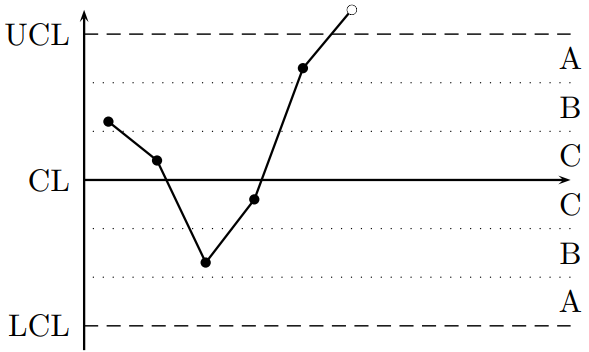
\includegraphics[width=\textwidth]{Pics/3.1.1.png}
%         \caption[Rule 1]%
%         {{\small Rule 1: Any point beyond zone A.}}
%         \label{fig:Rule 1}
%     \end{subfigure}
%     \hfill
%     \begin{subfigure}[b]{0.2\textwidth}
%         \centering
%         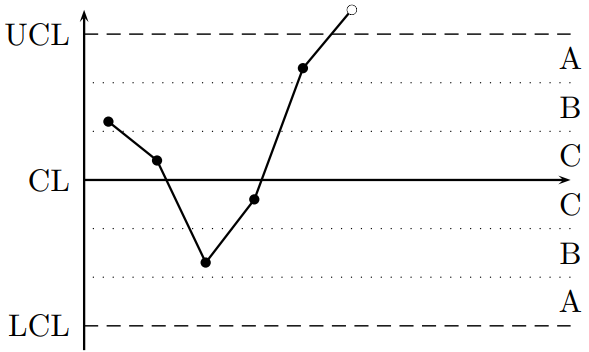
\includegraphics[width=\textwidth]{Pics/3.1.1.png}
%         \caption[Rule 2]%
%         {{\small Rule 2: Two out of three consecutive points fall on the same side in zone A or beyond.}}
%         \label{fig:Rule 2}
%     \end{subfigure}
%     % \vskip\baselineskip
%     \begin{subfigure}[b]{0.2\textwidth}
%         \centering
%         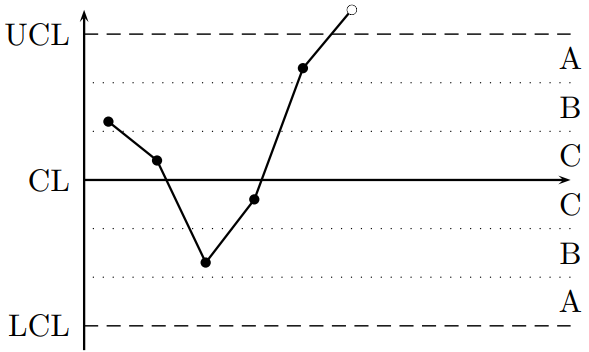
\includegraphics[width=\textwidth]{Pics/3.1.1.png}
%         \caption[Rule 3]%
%         {{\small Rule 3: Four out of five consecutive points fall on the same side in zone B or beyond.}}
%         \label{fig:Rule 3}
%     \end{subfigure}
%     \hfill
%     \begin{subfigure}[b]{0.2\textwidth}
%         \centering
%         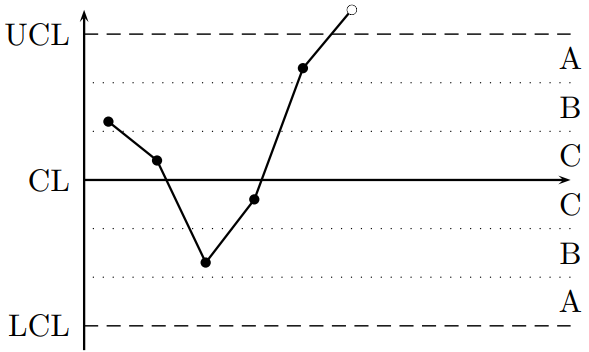
\includegraphics[width=\textwidth]{Pics/3.1.1.png}
%         \caption[Rule 4]%
%         {{Rule 4: Nine consecutive points fall on the same side of the centreline.}}
%         \label{fig:Rule 4}
%     \end{subfigure}
%     \caption[ The average and standard deviation of critical parameters ]
%     {\small The average and standard deviation of critical parameters: Region R4}
%     \label{fig:mean and std of nets}
% \end{figure*}

\subsection{Statistical Test}
\noindent\rule[\linienAbstand]{\linewidth}{\linienDicke}
Monitoring a production process with a control chart is equivalent to statistical testing.
\begin{equation}
  \begin{split}
    H_0:& \mu_0 = \mu \text{ i.e. process is not disturbed}\\
    H_1:& \mu_0 \neq \mu \text{ i.e. process is disturbed, } \mu_1 \text{ is true}
  \end{split}
\end{equation}
\textbf{Two wrong decisions possible:}\\
 - If a true null hypothesis $H_0$ is rejected we make a type $I$ error. An intervention in the process is necessary, because the control limits are exceeded, although the process is not disturbed. This is called a false alarm.\\
 - If a false null hypothesis $H_0$ is accepted we make a type $II$ error. There is no intervention, since the control limits are not exceeded, although the process is disturbed. This is called an omitted alarm\\

 \begin{table}[H]
   \setlength{\tabcolsep}{0em}
   \small
   \begin{tabular}{p{\linewidth / 2}p{\linewidth / 2}}
    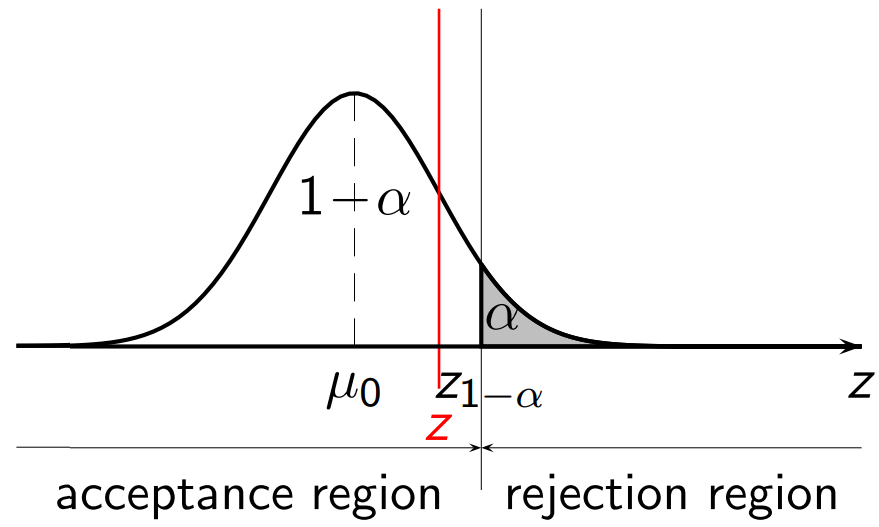
\includegraphics[width=\linewidth]{Pics/3.2.1.png}& 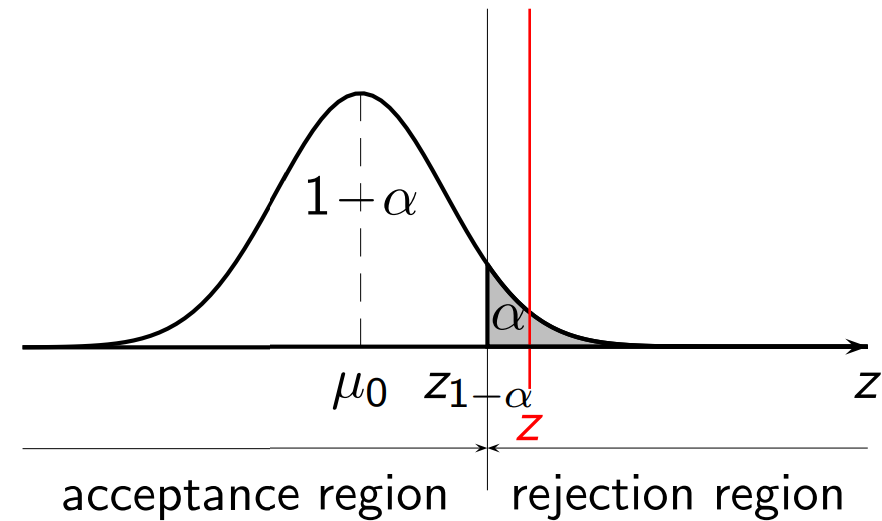
\includegraphics[width=\linewidth]{Pics/3.2.2.png} \\
    Let $h_0$ be true: Since $z < z_{1-\alpha}$ the null hypothesis is accepted. This is the right decision, which is made with probability $1-\alpha$. & Let $h_0$ be true: Since $z \geq z_{1-\alpha}$ the null hypothesis is rejected. This is the wrong decision (type $I$ error), which is made with probability $\alpha$.
  \end{tabular}
 \end{table}

\paragraph{Power Function}
% Power = 1 - beta = Probability to corretly reject H_0
% Power = g(mu_1) (also depends on n)
\begin{equation}
  g(\mu_1) = g(\delta\sigma + \mu_0) = G dach (\delta)
\end{equation}

Introduce delta
\begin{equation}
  \delta = \frac{\mu_1 - \mu_0}{\sigma}
\end{equation}
or $\mu_1 = \delta\sigma + \mu_0$


\paragraph{Process Capability}
\begin{equation}
  C_p = \frac{USL - LSL}{6\sigma}
\end{equation}

\begin{itemize}
  \item $C_p = 1$ implies a reject rate of $\alpha \cdot 100\% = 0.27\%$.
  \item $C_p < 1$ implies a reject rate of more than $\alpha \cdot 100\% = 0.27\%$, i.e. the process capability is not guaranteed.
  \item $C_p > 1$ implies a reject rate of less than $\alpha \cdot 100\% = 0.27\%$,i.e. the process capability is guaranteed.

\end{itemize}
